\documentclass{abnt}
\usepackage[brazil]{babel}
\usepackage[utf8]{inputenc}
\usepackage[num]{abntcite}
\usepackage{graphicx}
\usepackage{url}

\graphicspath{{imagens/}}

\begin{document}
\autor{André Taiar Marinho Oliveira}

\titulo{SAAS didático para um sistema de gestão estratégica}

\orientador[Orientador:\\]{Prof. Dr. Clarindo Isaías Pereira da Silva e Pádua}
\coorientador[Orientador:\\]{Prof. Dr. Marcelo Aureliano Monteiro de Andrade}

\comentario{Apresentado como de trabalho na disciplina de Atividades Práticas Integradoras do Curso de Bacharelado em Sistemas de Informação da UFMG}

\instituicao{Universidade Federal de Minas Gerais \par Instituto de Ciências
Exatas \par Departamento de Ciência da Computação}

\local{Belo Horizonte} \data{2015/2}

\capa
\folhaderosto

\begin{resumo}

Este trabalho tem como objetivo fundamentar os alicerces para a construção de um
produto dando embasamento teórico e a iniciação do desenvolvimento de um sistema
de gestão estratégica voltado para pequenas e médias empresas.

Em um sentido mais específico, a fundamentação seria mais precisamente na
integração de algumas ferramentas de gestão estratégica que compartilham entre
si dados comuns no contexto de uma organização. Como parte do projeto de
desenvolvimento do sistema, será preciso também utilizar conceitos de
engenharia de software para especificar e documentar os requisitos e
funcionalidades que serão fundamentais para o desenvolvimento do projeto.

Obteremos no final uma base teórica para guiar o desenvolvimento deste produto,
a especificação inicial do sistema que deseja-se desenvolver e um protótipo
mínimo da solução a ser desenvolvida.

\textbf{Palavras-chaves}: saas, gestão, estratégia, engenharia de software.
\end{resumo}

\sumario %comando que gera o sumário automaticamente
\renewcommand*\listfigurename{LISTA DE FIGURAS}
\listoffigures %comando que gera um sumário para a lista de figuras do texto automaticamente


\chapter{INTRODUÇÃO}

O planejamento estratégico das organizações surgiu em em meados da década de 60
se tratando de uma metodologia que permite estabelecer a direção a ser seguida
pela organização e visa um maior grau de interação com o ambiente aonde ela
atua. É um processo aonde se observa a organização por diversos ângulos,
direcionando os seus rumos e monitorando as suas ações de forma concreta.
Grandes empresas se beneficiam diretamente do planejamento através de gestão
estratégica de suas atividades, seja em um escopo amplo ou em projetos e sub
produtos dentro de sua cadeia de produção.

Micro e pequenas empresas não costumam se beneficiar diretamente do planejamento
estratégico e muitos motivos podem ser os motivos para que isso ocorra. O
assunto de Gestão Estratégica é bastante amplo; muitas técnicas podem ser
utilizadas e diversas análises podem ser feitas em cima de uma mesma organização
e dominar a utilização e entendimento destas ferramentas pode ser bastante
complicado para alguém não especialista na área. Mesmo que um gestor de
organização tenha domínio ou conhecimento específico sobre algumas destas
ferramentas do gerenciamento, utilizá-las parcialmente ou separadamente não é
tão efetivo quanto aplicá-las em uma sequência correta de passos com informações
integradas entre as etapas do processo. Além destes motivos, geralmente o gestor
de pequenas e médias empresas já tem grande parte do seu tempo tomado por
cumprir as funções do próprio metabolismo da organização, faltando tempo a ser
investido em conhecer melhor tais ferramentas e sua correta aplicação dentro do
cenário de sua organização.

A proposta desta monografia é desenvolver o protótipo de um sistema que agrupe
diversas ferramentas de gestão para planejamento estratégico de forma integrada.
A utilização destas ferramentas se dará de tal forma que o usuário do sistema
interaja com a plataforma seguindo um fluxo definido de atividades que se
integram e geram resultados mais relevantes em seu conjunto de especialidades.
Este fluxo de utilização deve ser o mais didático possível, permitindo que um
gestor de organização, independente de sua familiaridade com ferramentas de
gestão estratégica, consiga utilizar corretamente os conceitos e obter
informações para avaliação e direcionamento do negócio.

Espera-se que deste trabalho resulte um protótipo funcional que seja distribuído
como um Software as a Service (Saas) \cite{Turner2003}. A principal
característica em um software como serviço é a não aquisição das licenças mas
sim pagar pelo uso como um serviço. Funcionando em ambiente web, espera-se que
o modelo possibilite a aquisição do produto por um baixo preço, tornando sua
utilização viável para micro e pequenas empresas e atraindo mercado maior devido
a escala que pode alcançar.

\chapter{CONTEXTUALIZAÇÃO E TRABALHOS RELACIONADOS}

A temática deste trabalho é fortemente apoiada sob três pilares principais e
multidisciplinares. Primeiramente, será desenvolvido um sistema e isso será a
parte mais técnica do trabalho e reunirá conceitos de engenharia de software,
cloud computing e gerenciamento de projetos. Em segundo lugar, o software deve
implementar soluções para gerenciamento estratégico, abrangendo ferramentas
baseadas em teorias de gestão estratégica de organizações. Por fim, o sistema e
as informações devem ser disponibilizados por meio de uma interface intuitiva e
com forte apelo didático, apoiando o usuário às informações necessárias para
alimentar o sistema e, em alguns pontos críticos, instruindo o usuário na
operação que deve ser feita no sistema.

\section{Gestão estratégica}

% contextualização da gestão estratégica
O planejamento estratégico é considerado um instrumento administrativo
relacionado à estratégia empresarial, pois é a sustentação do desenvolvimento e
da implementação de estratégias empresariais \cite{OLIVEIRA1991}. 

Por definição, planejamento significa o desenvolvimento de um programa para a
realização de objetivos e metas organizacionais, envolvendo a escolha de um
curso de ação, a decisão antecipada do que deve ser feito, a determinação de
quando e como a ação deve ser realizada \cite{anaTerence}. 

A estratégia diz respeito à utilização dos recursos da organização que estão à
disposição de seu gestor \cite{ansoff1991nova}. Ao adotar uma estratégia, o
gestor analisar sua organização e o ambiente em que esta está inserido, para
decidir quais são os caminhos, os recursos e as ações que devem ser seguidos
para alcançar os objetivos previamente definidos \cite{anaTerence}.

% descrição básica dos módulos selecionados
O que chamamos neste trabalho de \textbf{ferramentas de gestão estratégica} se
refere a métodos, artefatos e regras que compõem um grupos de ferramentas de
gerenciamento de performance estratégica. No escopo do nosso produto, estas
ferramentas podem ser classificadas em seis grupos distintos:

\begin{itemize}
	\item Análise do negócio;
	\item Análise do mercado;
	\item Modelo de negócio;
	\item Planejamento estratégico;
	\item Análise de viabilidade econômica e financeira;
	\item Plano de ação.
\end{itemize}

Em nosso produto, estes grupos formariam a cadeia de análise e planejamento de
estratégia empresarial começando pelo posicionamento do negócio e passando
sequencialmente pelas ferramentas de análise do mercado, modelagem do negócio,
planejamento da estratégia, análise de indicadores e ferramentas de
acompanhamento e plano de ação.

Dentro de cada um destes grupos devem ser disponibilizadas diversas ferramentas.
Enumeraremos abaixo cada grupo e cada ferramenta que inicialmente deveria compor
o grupo.

\subsection{Ferramentas de Análise do negócio}

\begin{itemize}
	\item Diagrama Empresarial \cite{DiagramaEmpresarial}
	\item Curva de Valor \cite{CurvaValor}
	\item Matriz BCG \cite{BCG}
	\item Análise SWOT \cite{SWOT}
	\item Cadeia de Valor \cite{CadeiaDeValor}
\end{itemize}

\subsection{Ferramentas de Análise do mercado}

\begin{itemize}
	\item Forças do Mercado \cite{Porter}
	\item Forças Macroeconômicas \cite{Porter}
	\item Forças da Indústria \cite{Porter}
	\item Tendências principais \cite{Porter}
\end{itemize}

\subsection{Ferramentas de Modelo de negócio}

\begin{itemize}
	\item Canvas Model \cite{Canvas}
	\item Padrões de Modelo de Negócio \cite{ModeloNegocio}
	\item Ambiente de Modelo de Negócio \cite{AmbienteNegocio}
	\item Avaliação de Modelo de Negócio \cite{Canvas}
\end{itemize}


\subsection{Ferramentas de Planejamento estratégico}

\begin{itemize}
	\item Balanced Scorecard \cite{BSC}
	\item Mapa Estratégico \cite{MapaEstrategico}
	\item Gerenciamento por Diretrizes \cite{GerDiret}
\end{itemize}

\subsection{Ferramentas de Análise de viabilidade econômica e financeira}

\begin{itemize}
	\item Projetar retorno sobre investimento \cite{RetInvest}
	\item Indicador de EBITDA \cite{Ebitda}
	\item Indicador de Lucratividade \cite{Lucratividade}
	\item Cálculo de Fluxo de Caixa Projetado \cite{FluxoCaixa}
	\item Cálculo de TIR \cite{TIR}
	\item Cálculo de VPL \cite{VPL}
\end{itemize}

\subsection{Ferramentas de Plano de ação}

\begin{itemize}
	\item 5W2H \cite{5W2H}
	\item Cronograma e Workflow \cite{Crono}\cite{WorkFlow}
	\item OKR \cite{OKR}
	\item Kanban \cite{Kanban}
\end{itemize}

% explicar o gráfico e exemplificar um modelo de fluxo no sistema

\begin{figure}[!htb]
	\centering
	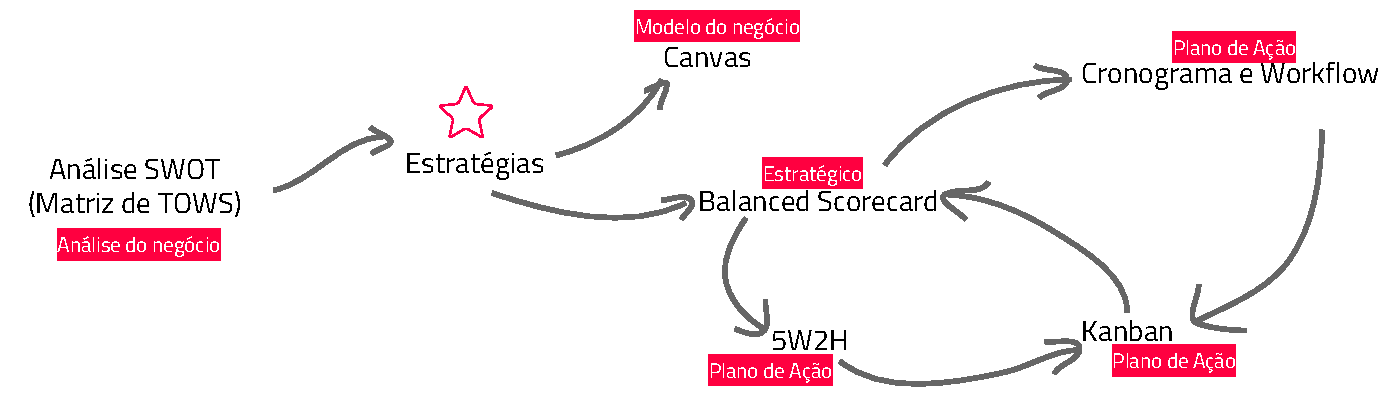
\includegraphics[width=\textwidth]{fluxograma_exemplo.pdf}
	\caption{Exemplo de fluxo de trabalho possível no sistema}
	\label{Rotulo}
\end{figure}

\section{Didática}

% validar a idéia de facilidade de uso do sistema com relação à usuários leigos
% adicionar ideias de interação e ajudo do sistema
% validar coisas através de IHC

\section{Software (as a Service)}

% contextualizar o software como serviço
% contextualizar as metodologias que serão utilizadas

\chapter{DESENVOLVIMENTO DO TRABALHO}

\section{Proposta e projeto do sistema}

% relacionar ferramentas utilizadas e tecnologia
% explicar a aplicação da metodologia

\section{Desenvolvimento do projeto}

% mostrar diagramas
% mostrar histórias de usuários
% falar sobre as sprints

\chapter{RESULTADOS E DISCUSSÃO}

% apresentação da solução criada (precisa ter o BSC)

\chapter{CONCLUSÕES E TRABALHO FUTUROS}

O projeto de interação entre os módulos do sistema demonstrou-se com o tempo ser
extremamente mais oneroso do que o que foi estimado no início do projeto. Também
é visível que o plano inicial de desenvolver muitos módulos e ferramentas de
gestão seria inviável ao longo de um semestre letivo. Neste ponto, a metodologia
ágil que foi escolhida para gerenciamento do projeto ajudou a refinar as tarefas
que existiam no \textit{backlog} do projeto, priorizando o que provavelmente
daria mais visibilidade ao projeto e que poderia ser relevante no contexto de um
sistema de gestão estratégica: o módulo de \textit{Balanced Scorecard}.

% TODO: falta algum elemento intermediário

Um produto mínimo viável como o que foi idealizado nesse trabalho parece ter um
potencial de crescimento muito grande. Como visto, o fluxo do projeto idealizado
foi muito grande em relação ao o que consegui desenvolver ao longo de um
semestre letivo. Por se tratar de um projeto com um certo apelo comercial,
pretendo continuar desenvolvendo o produto e investir mais esforço na produção
de um sistema mais completo.


\bibliography{bibliog}

\end{document}
